%%%%%%%%%%%%%%%%%%%%%%% file tdp-draft.tex %%%%%%%%%%%%%%%%%%%%%%%%
%
% TDP Draft version 
% Created by Krit
%
%%%%%%%%%%%%%%%%%%%%%%%%%%%%%%%%%%%%%%%%%%%%%%%%%%%%%%%%%%%%%%%%%%%

\documentclass{llncs}

\usepackage{url}
\usepackage{amsmath}
\usepackage{array}
\usepackage{graphicx}
\usepackage{color}

\newcommand{\dq}[1]{``#1''}
\newcommand{\dit}[1]{\dq{\textit{#1}}}
\newcommand{\md}[1]{\(#1\)}
\newcolumntype{C}[1]{>{\centering\let\newline\\\arraybackslash\hspace{0pt}}m{#1}}

\begin{document}

\title{SKUBA 2016 Team Description}
\author{Kandith Wongsuwan
\and Krit Chaiso
\and Nut Kaewnak
\and Konlayut Songkrasin
\and Nathas Yingsukamol
\and Thanachote Visetsuthimont
\and Kanjanapan Sukvichai
}

\institute{ Faculty of Engineering, Kasetsart University\\
50 Ngamwongwan Rd, Ladyao, Bangkok, Thailand\\
\email{skuba2002@gmail.com}\\
\url{http://iml.cpe.ku.ac.th/skuba}
}

\maketitle

\begin{abstract}
This paper briefly describes software architecture and hardware design of a household service robot developed by SKUBA, an intelligent robotic team from Kasetsart University, Thailand, in order to participate in Robocup@Home 2016 at Leipzig, Germany. As the robot hardware satisfy our minimum requirements, this year the research mainly focuses on improving the software system. Object Recognition, Speech Recognition, and Manipulation modules \textemdash\ which are main problems from our lastest competition \textemdash\ have been developed in its efficacy. Clothing Type Classification is implemented to serve human in a real-life application. This year, we will evaluate our new techniques in contesting environment.

\end{abstract}

\section{Introduction}

Robots always fascinate humans, especially a human-like robot. Most of the robot mechanisms are replicas of human body or human parts, for instance, legs and arms. Humans always create a robot that manipulates human activities in order to help human doing thier jobs. A housekeeping robot is an interesting topic in researches worldwide due to its intricated mechanism and artificial intelligence. SKUBA@Home was established in 2011. The aim of SKUBA@Home is to develop the housekeeping robot that can help human in real-time and real-life applications. The first robot is developed in 2012. We joined Robocup Japan Open 2012, and made the way through the finalist. SKUBA@Home robot was continuously improved and joined the Robocup since 2012. The latest robot platform was designed in 2015 by improving robot mechanism, electronics and especially the robot's intelligent system. We joined RoboCup Japan Open and Robocup 2015 and passed to the second state from both competitions. 

In this year, there are three major improvements on our robot’s software system. First, Object Recognition module is re-implemented in order to improve the performance and the speed. Second improvement is Speech Recognition module. Multi-grammars models were implemented in our system then robot system can change the grammars in real-time operation. The last implementation is the Clothing Type Classification module. This module had an idea of the real-life application for a housekeeping robot. Therefore, our goal of this research is that the robot can tell the target apparel type.

\section{Robot Hardware} 
Our robot platform can be divided into three parts. The first part is the robot base. In order to make a precise movement, less mechanical slip and less vibration, four 6" aluminum mecanum wheels are used. Each wheel is driven by 70 watt Maxon Brushless DC (BLDC) motor, combined with planetary 19:1 gearhead ratio. The FPGA Spartan III is chosen to be the main controller in order to drive four brushless motors synchronously. The Hokuto laser length finder (URG-04Lx-UG01) is attached to the front of the base to gather surrounding information for the navigation system.

The second part is the robot arm and torso. Shoulder and elbow joints are controlled by high-torque DC motors with absolute encoder attached. In addition, the robot’s wrist and gripper joints are required less torque, therefore, one Dynamixel RX-64 and two Dynamixel Rx-28 servos are chosen as actuators. By combining all of the actuator's motions, the arm can move freely in 6 degrees of freedom. To make the robot height adjustable, the robot’s upper body is attached to a ball screw and linear guide supports.
    
The final part is the robot head. The robot head is moved by robot neck which has two degrees of freedom simulating human neck motion. The RODE microphone, Kinect Sensor, and Logitech C920 HD webcam are installed at the robot head which can be used as an anthropomorphic head. Due to the low image quality of Kinect's RGB camera, HD webcam is substituted. To acquire the projection between the webcam and Kinect axis, normal camera calibration algorithm does not work properly because of noisy depth data. The problem is solved by finding the transformation between webcam and Kinect's RGB. Then it is biased with a constant distance value between depth sensor and Kinect's RGB camera to facilitate the camera’s calibration process.

\begin{figure}
\centering
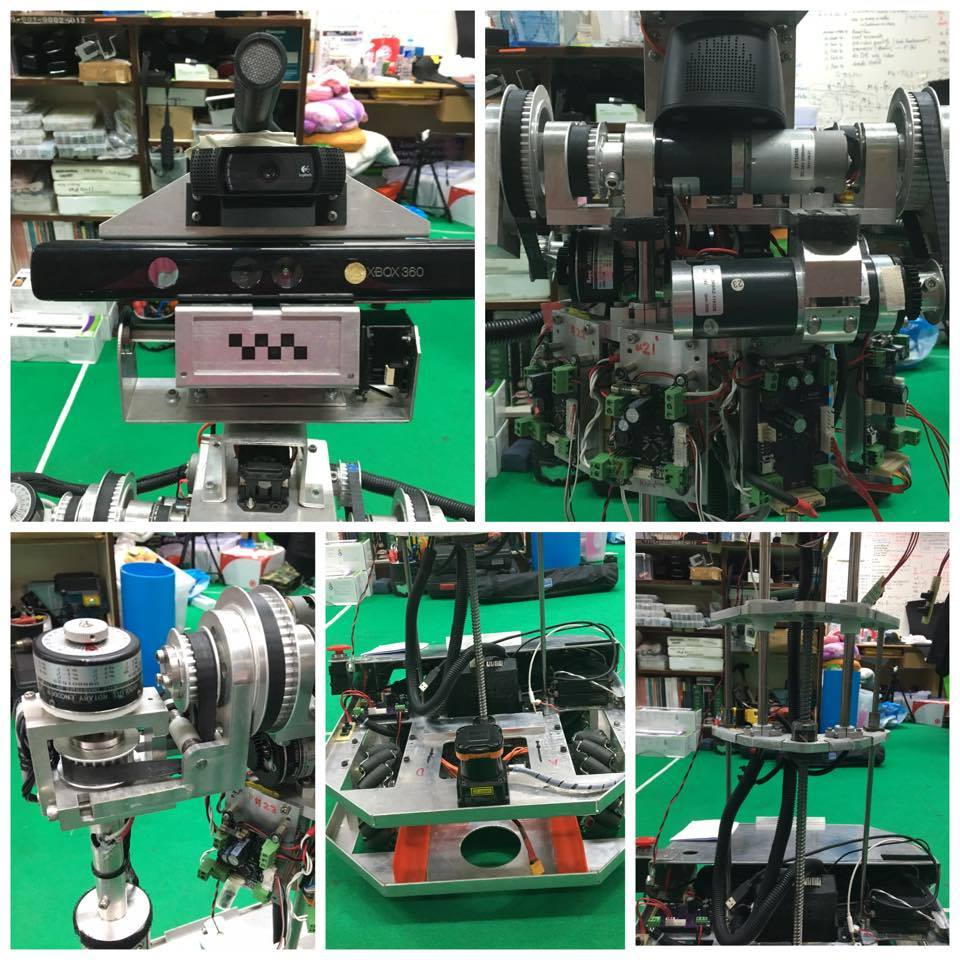
\includegraphics[width=9cm, height=6cm]{realrobot}
\caption{Our robot design.}
\label{fig:base}
\end{figure}

\section{Software Architecture}
The software system of our robot is separated by its functionality into modules, for example, an object recognition module, a planning module. Each module communicates through Robot Operating System (ROS). Modules can be organized into three different layers:   \textit{Perception Layer}, \textit{Control Layer} and \textit{Decision Layer}.

\textit{Perception Layer} consists of modules that process about environmental understanding.  Speech recognition, Object recognition, and Localization, for instance. Modules in this layer collect various data from sensors, i.e., laser rangefinder, microphone, Kinect, and webcam, to perform higher-level algorithms in order to identify the state of the environment. The output from this layer is intermediate data for \textit{Decision Layer}.

\textit{Decision Layer} controls robot's behavior to solve complicated tasks. In this layer, decision is made based on information from perception layer and the user's command. The command is classified into three categories: \textit{question}, \textit{command} and \textit{informative}. \textit{Question} is a sentence which the user expects to get a proper answer from the robot. \textit{Command} is used when the user wants the robot to perform an action, for example, \dq{Bring me a pringle} and \dq{Follow me}. When the robot gets an information, such as \dq{My name is Brian} and \dq{This is kitchen}, these sentences will be classified as the \textit{Informative command}. 

When \textit{Decision Layer} sends command to the robot, \textit{Control Layer} will interpret those commands into lower-level actions by using path planning algorithms. Furthermore, the layer also controls robot manipulator with precision.

\subsection{Speech Recognition}

In this year, we adjust the speech recognition system to be adaptable based on Pocketsphinx, an open source speech recognition toolkit from Carnegie Mellon University (CMU). By creating the top-layer state decision module to control the speech recognition system, we are able to enable, disable, or change the Grammar, Language Model and Dictionary. Thus, we can adapt voice detection components freely, depending on the situation.
 
In addition, we developed an auto-generated grammar tools to generate the grammar from a set of sentences based on general trees. In order to optimize the grammar, a General Tree is used to separate a sentence into words, and reduces duplicated nodes simultaneously. Then, words are transformed into a tree structure. Consequently, the grammar file is generated from the tree.

\subsection{Object Recognition}
    
For object recognition, we change an implementation approach in order to improve the overall performance and increase the processing speed. Our last implementation, the extracted SURF descriptors are clustered by using K-means clustering. Then, the histogram for each object is created by counting the number of descriptors in each cluster \cite{obj_rec_surf}. However, this method takes loads of calculation time to match features in K-means clustered features dictionary.
 
New method is proposed this year. Histogram of Oriented Gradients (HOG) and a linear kernel Support Vector Machine (SVM) classifier is used in object recognition. Firstly, we prepare a dataset to train an object classifier as described in \cite{traininghaar}, where half of generated training data is positive (contains target objects) and the other half is negative (arbitrary images without target objects). Then, HOG features are extracted from each of training samples in the size of 8x8 local patches, which are used as a feature vector to train the object classifier model. To perform object detection and recognition, we use 2D images acquired from the webcam. We apply a multi-scale window search algorithm to the image and then perform an object classification using HOG and the trained SVM model in each window. Therefore, the object with above the SVM’s confidence threshold is detected and localized. Finally, the detected object location in the image is mapped back to the robot workspace with a 3D point cloud. The result of our proposed approach is shown in Fig.\ref{fig:objectHOG}

\begin{figure}
\centering
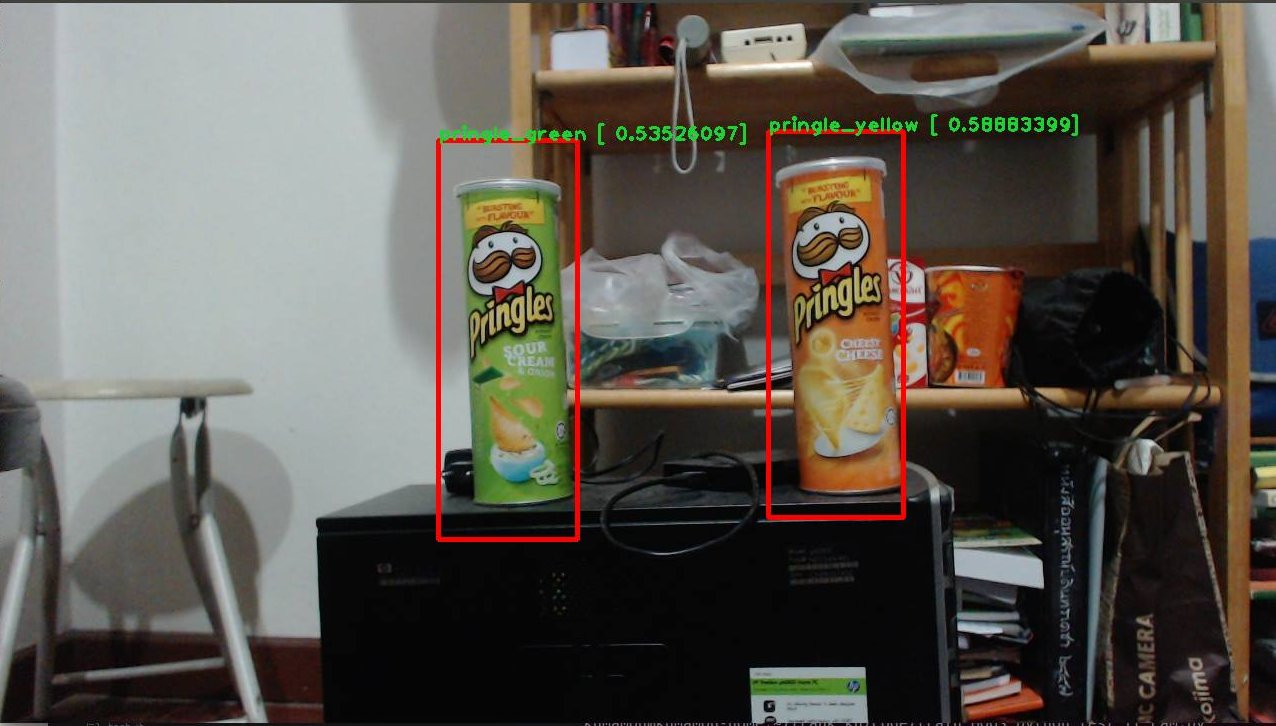
\includegraphics[height=5.2cm]{object_hog}
\caption{Result from object recognition module}
\label{fig:objectHOG}
\end{figure}

\subsection{Clothing Classification}

People distinguish and recognize types of clothes in their daily routine for various applications. For instance, we separate types of clothes for laundry, which is needed to be treated differently, or even recommending styles to each other. 

For a household service robot, Clothing Type Classification is an interesting and useful task, yet a challenging topic to perform since there is no specific attribute to determine each type of apparel. Therefore, our goal of this research is that the robot can tell the target apparel type whether it is shorts, jeans, underwear, shirt, T-shirt, blouse or jacket.	 
 
In practice, we provided that unfolded pieces of clothes are lying on a flat planar. First, in the localization process, we localize the planar surface in a RGB-D point cloud using \cite{pcllib} plane segmentation, and extract its RGB image. In order to localize clothes on the plane, Efficient Graph-Based Image Segmentation \cite{egbis} is used to separate non-rigid objects and background. After localizing objects, we extract features including Speeded up robust features(SURF), HOG, and L*a*b* color histogram from each image segment, then features vectors are quantized using KMeans. Finally, each quantized features vectors are concatenated and a one-versus-all linear SVM is used as a classifier for each clothing type category. The SVM model is trained using the dataset from \cite{apparel_with_style} and some additional Google queried data. The result of the implemented procedure is shown in Fig.\ref{fig:clothtype}

\begin{figure}
\centering
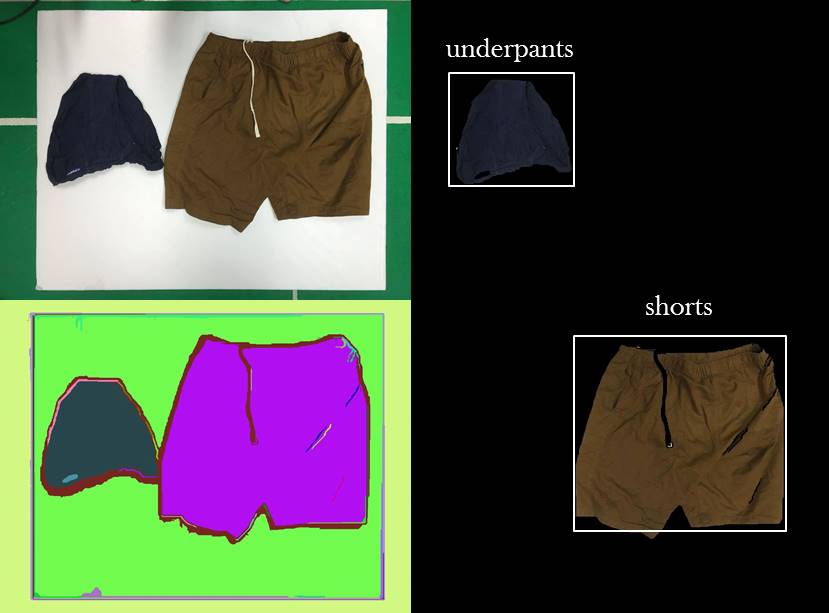
\includegraphics[width=10cm,height=5.2cm]{ClothType}
\caption{(Top-Left) An Input Image, (Bottom-Left) Plane Localization and Efficient Graph-Based Image Segmentation, (Right) Output Results}
\label{fig:clothtype}
\end{figure} 

\section{Motion Control and Planning}

\subsection{Motor Control System}

Control system is separated into two modules, a base and arm module. The base controller uses FPGA embedded board to handle the base which consists of four mecanum wheels. PI velocity controller is implemented for each wheel. The serial communication (RS232) is used to communicate between FPGA and computer. The second module, arm controller, uses customized embedded board in order to handle DC motors of robot joints. In order to control the arm position, PID controller is implemented and an absolute encoder is chosen to gather absolute joint angle value. For precise rotation of a wrist and gripper, Dynamixel servo motors are used to control the motion and communicate with host computer via RS485 \cite{con_arm}.

\subsection{Localization and Path Planning}

Adaptive Monte Carlo Localization system (AMCL), provided by \textit{navigation} stack, is used for robot localization. To serve localization algorithm, Hokuyo laser length finder which acquires environmental data is attached to the robot. Additionally, the robot odometry information is also considered as one input information to localization algorithm. Another input is the known map, shown in Fig.\ref{fig:hector}, which is statically or dynamically construct. From previously describe input, AMCL which is a particle filter localization system accurately estimates position and orientation of the robot.

\begin{figure}
\centering
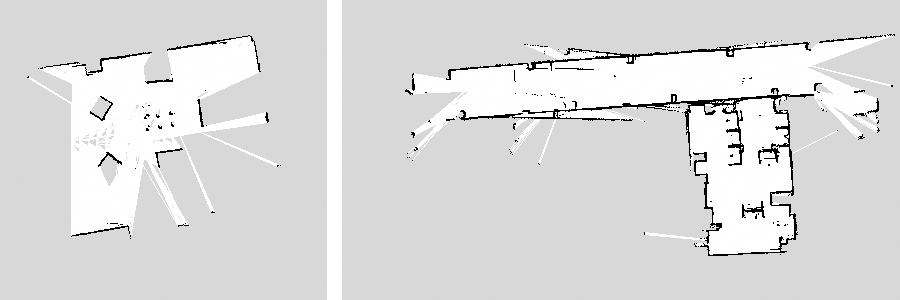
\includegraphics[height=3.9cm]{hector_map}
\caption{Occupancy map from \textit{hector\_mapping}}
\label{fig:hector}
\end{figure}

To achieve path planning, there is \textit{move\_base} node in \textit{navigation} stack that is consist of two types of planning method. Begin with global planner, this method provides an effective path for robot to navigate through the known map. By using Dijkstra's algorithm, the result path is the shortest and acceptable. Then local planner method move to destination following designated path and avoid obstacles along the way. In order to move robot, local planner determine its velocity and orientation. This node directly send command to the robot.

\subsubsection{Odometry Estimation Module}

This module helps to minimize the mean square error of the non-perfect sensor measurement originated from wheel slippage, noises surrounding environment and IMU drift over time. Using the laser scanner to estimate the change of position, with laser scan matching technique, can solve the wheel slip problem while facing with high sensitivity and dynamic environment. Point-to-line distance Iterative Closed Point (ICP) method is used to be based algorithm for laser scan matching.

To perform the estimation module, A Kalman filter, which consists of two steps, is used. First, the Kalman's observation step calculates difference between output from last prediction and actual position which combine laser scan matching and wheels' speed together. Next, the Kalman's prediction step predicts new output by compensate error from the previous step and IMU data\cite{odom}.

\subsubsection{Collision Avoidance Module}

This component ease the planning module to organize safety movement. By retrieving point cloud data from Kinect, this module projects each point to occupancy map. In order to avoid obstacles, path planner retrieves projection data and manages to construct smooth path. Due to unusual data, such as, ground plane and wall partition, planar elimination algorithm is applied. Result data from algorithm, for instance, table and chair, is projected and pass to planning module continuously\cite{avoid}.

\subsection{Manipulation Module}

To excel performance in picking and grasping objects, in this year, the manipulation module is reimplemented based on Moveit!, the state of the art software for mobile manipulation. In our last implementation, inverse kinematic equations were solved in mathematical closed-form in hardware-limited conditions.  The equations set, however, cannot perform dynamic arm’s trajectory planning. For example, generated paths were not able to avoid the robot itself, or obstacles in front of the robot, in turn, it was failed to reach its goal and also caused damages to the hardware. The new manipulation system based on Moveit! can dynamically generate trajectories, which are able to avoid the obstacles, using the Open Motion Planning Library (OMPL). In addition, the system is able to perceive obstacles and target objects in robot workspace through collision map in RVIZ \textemdash\ 3D visualization tools in ROS. This collision map is created from others scene processing ROS node, e.g., octomap, object recognition node. Consequently, we can improve overall manipulation module performance and prepare a structure for further development in advanced manipulation system.
\begin{figure}
\centering
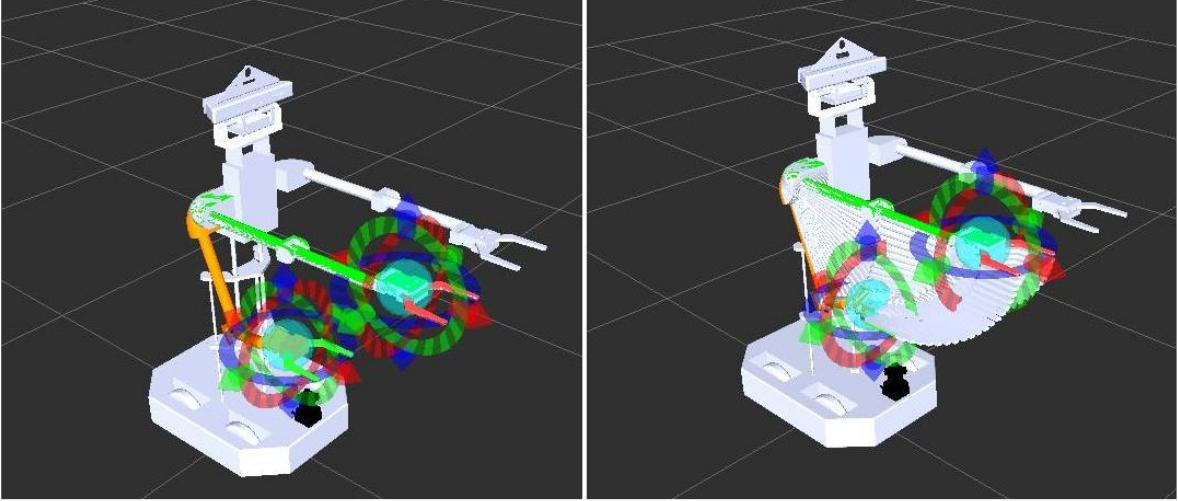
\includegraphics[width=12cm, height=5cm]{Moveit}
\caption{Generated Trajectory using Moveit! and RVIZ Visulization}
\label{fig:moveit}
\end{figure} 


\section{Conclusion}

Our main improvements for our robot this year are Object Recognition, Speech Recognition, Clothing Type Classification and Manipulation motion. The robot mechanism remains the same as last year but its major improvement is in manipulator planing algorithm, as well as object classifier. Clothing Type Classification is added to the robot system in order to improve robot capability to help human in a real-life application. From lessons-learned in our latest competition leads us to discover new development ideas in order to improve our robot. For Robocup 2016 in Germany, our robot is more sophisticated and ready to participate the competition. We hope that SKUBA will surpass our performance in last year RoboCup, and we are looking forward to sharing experiences with other great teams from all around the world.

\section*{Team Member}

This year, SKUBA@Home team consists of these following members:
\begin{itemize}
\item Supervisor, Financial Support: Kanjanapan Sukvichai
\item Team Leader: Nut Kaewnak
\item Computer Engineering: Krit Chaiso, Nathas Yingsukamol, Pattaraporn Tulathum, Thanachote Visetsuthimont and Nutthaphon Thamrapeepithak 
\item Electrical Engineering:  Kandith Wongsuwan, Konlayut Songkrasin, Teeratath Ariyachartphadungkit, and Pruttapon Maolanon
\item Mechanical Engineering: Surachat Chantarachit, and Vasuwat Kittiwangchai
\end{itemize}
\begin{thebibliography}{4}

\bibitem{con_arm} T. Ariyachartphadungkit and K. Sukvichai, Development of an Embedded BLDC motor controller using RS485 standard, 2013.

\bibitem{obj_rec_surf} D. Schmitt and N. McCoy. Object Classification and Localization Using SURF Descriptors. 2011.

\bibitem{hector_slam} S. Kohlbrecher and J. Meyer and O. von Stryk and U. Klingauf. A Flexible and Scalable SLAM System with Full 3D Motion Estimation, in Proc. IEEE International Symposium on Safety, Security and Rescue Robotics (SSRR), November, 2011.

\bibitem{odom} B. Pholpoke and K. Sukvichai. Real Time People Tracking and Collision Avoidance using Sensors Fusion for an Indoor Omni-directional Wheels Mobile Robot, 2013.

\bibitem{avoid} T. Chaveekolakit and K. Sukvichai. Development of Ground Planar Segmentation algorithm using 3D Point Clouds Information from Kinect Depth Image Camera, 2013.

\bibitem{egbis} P. F. Felzenszwalb and D. P. Huttenlocher. Efficient Graph-Based Image Segmentation. International Journal of Computer Vision, 2004, 59.2: 167-181.

\bibitem{apparel_with_style} L. Bossard, et al. Apparel classification with style. In Computer Vision–ACCV 2012 (pp. 321-335). Springer Berlin Heidelberg.

\bibitem{pcllib} R. B. Rusu,  and S. Cousins. 3d is here: Point cloud library (pcl). In Robotics and Automation (ICRA), 2011 IEEE International Conference on (pp. 1-4). IEEE.

\bibitem{traininghaar} N. Seo. Tutorial: OpenCV haartraining (Rapid Object Detection With A Cascade of Boosted Classifiers Based on Haar-like Features). note.sonots.com

\end{thebibliography}

\end{document}
